% ============================================================
%  PopsUp — AI HR Onboarding Workflow Orchestrator
%  IBM Hackathon Submission · 3-Page Technical Report
%  Compile on Overleaf (pdfLaTeX, no extra packages needed)
% ============================================================
\documentclass[10pt,a4paper]{article}

% ── Packages ────────────────────────────────────────────────
\usepackage[top=2cm,bottom=2cm,left=2.2cm,right=2.2cm]{geometry}
\usepackage{graphicx}
\usepackage{xcolor}
\usepackage{fontenc}
\usepackage{inputenc}
\usepackage{lmodern}
\usepackage{microtype}
\usepackage{titlesec}
\usepackage{enumitem}
\usepackage{tabularx}
\usepackage{booktabs}
\usepackage{multicol}
\usepackage{mdframed}
\usepackage{tikz}
\usepackage{fancyhdr}
\usepackage{hyperref}
\usepackage{parskip}
\usepackage{array}
\usepackage{colortbl}

% ── IBM colour palette ───────────────────────────────────────
\definecolor{IBMBlue}{HTML}{0F62FE}
\definecolor{IBMDark}{HTML}{001141}
\definecolor{IBMLight}{HTML}{D0E2FF}
\definecolor{IBMGray}{HTML}{F4F4F4}
\definecolor{IBMMid}{HTML}{6F6F6F}
\definecolor{AccentGreen}{HTML}{24A148}
\definecolor{AccentPurple}{HTML}{6929C4}

% ── Section styling ─────────────────────────────────────────
\titleformat{\section}
  {\large\bfseries\color{IBMBlue}}
  {}
  {0em}
  {}[\color{IBMBlue}\titlerule]

\titleformat{\subsection}
  {\normalsize\bfseries\color{IBMDark}}
  {}
  {0em}
  {}

\titlespacing{\section}{0pt}{10pt}{4pt}
\titlespacing{\subsection}{0pt}{6pt}{2pt}

% ── Header / Footer ─────────────────────────────────────────
\pagestyle{fancy}
\fancyhf{}
\renewcommand{\headrulewidth}{0pt}
\fancyhead[L]{\small\color{IBMMid}\textbf{PopsUp} · AI HR Onboarding Orchestrator}
\fancyhead[R]{\small\color{IBMMid}IBM Hackathon Submission}
\fancyfoot[C]{\small\color{IBMMid}\thepage}

% ── Helpers ─────────────────────────────────────────────────
\newcommand{\badge}[2]{%
  \tikz[baseline=-0.6ex]\node[fill=#1,text=white,rounded corners=3pt,
    inner xsep=5pt,inner ysep=2pt,font=\scriptsize\bfseries]{#2};}

\newmdenv[
  backgroundcolor=IBMGray,
  linecolor=IBMBlue,
  linewidth=1.2pt,
  leftline=true, rightline=false, topline=false, bottomline=false,
  innerleftmargin=8pt, innerrightmargin=6pt,
  innertopmargin=5pt, innerbottommargin=5pt,
  skipabove=6pt, skipbelow=4pt
]{sidebox}

% ── Image placeholder helper ────────────────────────────────
% Usage: \screenshot{width}{caption text}
\newcommand{\screenshot}[2]{%
  \begin{center}
  \begin{tikzpicture}
    \draw[fill=IBMGray, draw=IBMBlue, line width=0.8pt, rounded corners=4pt]
      (0,0) rectangle (#1, 4.2cm);
    \node[color=IBMMid, font=\small] at (#1/2, 2.1cm) {%
      \begin{tabular}{c}
        \includegraphics[width=1cm]{example-image}\\[2pt]
        \textit{[ #2 ]}
      \end{tabular}
    };
  \end{tikzpicture}
  \end{center}
}

% ────────────────────────────────────────────────────────────
\begin{document}

% ════════════════════════════════════════════════════════════
%  TITLE BLOCK
% ════════════════════════════════════════════════════════════
\begin{tikzpicture}[remember picture, overlay]
  \fill[IBMDark] (current page.north west)
    rectangle ([yshift=-3.6cm]current page.north east);
\end{tikzpicture}

\vspace*{0.3cm}
{\color{white}
  \hspace{0.1cm}
  \begin{minipage}{0.68\textwidth}
    {\fontsize{22}{26}\selectfont\bfseries PopsUp}\\[3pt]
    {\large\bfseries AI HR Onboarding Workflow Orchestrator}\\[6pt]
    {\small IBM Hackathon Submission · Technical Project Report}
  \end{minipage}
  \hfill
  \begin{minipage}{0.28\textwidth}\raggedleft
    \badge{IBMBlue}{IBM watsonx.ai}\\[4pt]
    \badge{AccentGreen}{RAG Pipeline}\\[4pt]
    \badge{AccentPurple}{FastAPI + React}
  \end{minipage}
  \hspace{0.1cm}
}
\vspace{0.7cm}

% ════════════════════════════════════════════════════════════
%  PAGE 1
% ════════════════════════════════════════════════════════════

% ── Two-column abstract row ─────────────────────────────────
\begin{multicols}{2}

\section{Problem Statement}

HR onboarding is one of the most time-consuming, error-prone, and inconsistent
processes in any large organisation. Policy documents are scattered across shared
drives; new hires receive different information depending on who onboards them;
and HR teams spend hours manually answering the same questions repeatedly.

The cost is measurable: studies show that a poor onboarding experience increases
early attrition by up to \textbf{20\%}, and the average cost of replacing an
employee exceeds \textbf{50\% of their annual salary}. For a company of 1,000
employees with 15\% annual turnover, this represents millions of dollars in
preventable loss.

\columnbreak

\section{Solution Statement}

\textbf{PopsUp} is an AI-powered HR onboarding orchestrator that turns static
policy documents into intelligent, interactive, and role-specific onboarding
experiences.

HR teams upload their existing PDF or DOCX policy documents. The system
automatically ingests, indexes, and understands them using a
\textbf{Retrieval-Augmented Generation (RAG)} pipeline backed by IBM
\textbf{watsonx.ai} (Granite). Employees and HR managers can then:

\begin{itemize}[leftmargin=1em,itemsep=1pt]
  \item \textbf{Ask questions} in plain English and receive contextually
        accurate answers sourced directly from company policy.
  \item \textbf{Generate personalised onboarding workflows} tailored to a
        specific role or department — structured, actionable, and exportable.
  \item \textbf{Track and approve} each onboarding step through an interactive
        timeline with Approve / Reject / Complete controls.
\end{itemize}

The result: consistent, scalable, and measurable onboarding — without any
manual effort after the initial document upload.

\end{multicols}

% ── Architecture diagram ─────────────────────────────────────
\section{System Architecture}

\begin{center}
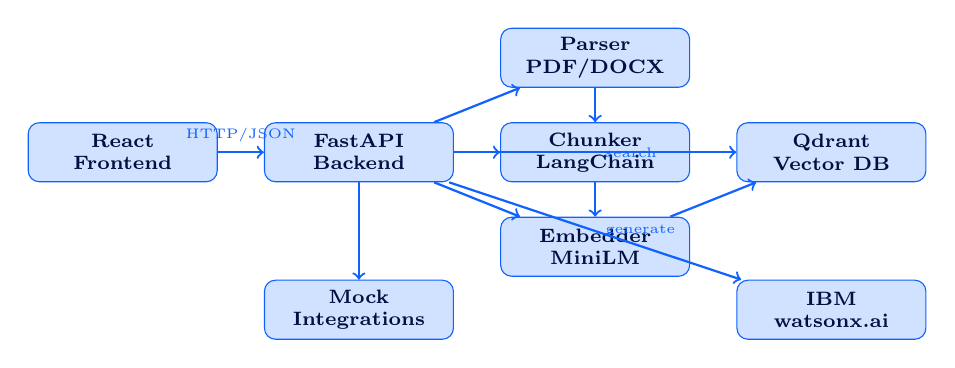
\begin{tikzpicture}[
  box/.style={draw=IBMBlue, fill=IBMLight, rounded corners=4pt,
              minimum width=2.4cm, minimum height=0.75cm,
              font=\scriptsize\bfseries, text=IBMDark, align=center},
  arrow/.style={->, thick, color=IBMBlue},
  label/.style={font=\tiny\color{IBMMid}, align=center}
]
  \node[box] (ui)       at (0,0)    {React\\Frontend};
  \node[box] (api)      at (3,0)    {FastAPI\\Backend};
  \node[box] (parser)   at (6,1.2)  {Parser\\PDF/DOCX};
  \node[box] (chunker)  at (6,0)    {Chunker\\LangChain};
  \node[box] (embedder) at (6,-1.2) {Embedder\\MiniLM};
  \node[box] (qdrant)   at (9,0)    {Qdrant\\Vector DB};
  \node[box] (watsonx)  at (9,-2)   {IBM\\watsonx.ai};
  \node[box] (integ)    at (3,-2)   {Mock\\Integrations};

  \draw[arrow] (ui) -- node[above,label]{HTTP/JSON} (api);
  \draw[arrow] (api) -- (parser);
  \draw[arrow] (api) -- (chunker);
  \draw[arrow] (api) -- (embedder);
  \draw[arrow] (parser) -- (chunker);
  \draw[arrow] (chunker) -- (embedder);
  \draw[arrow] (embedder) -- (qdrant);
  \draw[arrow] (api) -- node[right,label]{search} (qdrant);
  \draw[arrow] (api) -- node[right,label]{generate} (watsonx);
  \draw[arrow] (api) -- (integ);
\end{tikzpicture}
\end{center}

\vspace{-2pt}
\begin{center}
{\scriptsize\color{IBMMid}
\textbf{Upload flow:} File → Parser → Chunker → Embedder → Qdrant \quad
\textbf{Query flow:} Question → Embed → Qdrant Search → watsonx.ai → Answer}
\end{center}

% ── Tech stack table ────────────────────────────────────────
\vspace{4pt}
\begin{tabularx}{\textwidth}{>{\bfseries\color{IBMDark}}l X}
\toprule
\rowcolor{IBMLight}
\textbf{Layer} & \textbf{Technology} \\
\midrule
Frontend      & React 18, TypeScript, Vite, TailwindCSS \\
Backend       & FastAPI, Python 3.12, Pydantic v2 \\
AI / LLM      & IBM watsonx.ai — Granite 13B Instruct v2 (swappable via \texttt{AIProvider}) \\
Embeddings    & sentence-transformers \texttt{all-MiniLM-L6-v2} (384-dim cosine similarity) \\
Vector DB     & Qdrant — cosine similarity, collection-per-deployment \\
Document Parsing & PyMuPDF (PDF), python-docx (DOCX) \\
Orchestration & LangChain \texttt{RecursiveCharacterTextSplitter} (512 tok, 64 overlap) \\
Deployment    & Docker Compose — three services: frontend, backend, qdrant \\
\bottomrule
\end{tabularx}

\newpage

% ════════════════════════════════════════════════════════════
%  PAGE 2 — Features + Screenshots
% ════════════════════════════════════════════════════════════

\section{Core Features \& User Interface}

\subsection{1 · Document Upload \& Ingestion}

Users drag-and-drop PDF or DOCX HR policy documents. The backend immediately
runs a five-stage ingestion pipeline: \textbf{save → extract text → chunk →
embed → upsert into Qdrant}. The upload page displays every document currently
stored in the vector store with its chunk count, and includes a one-click
\emph{Load Sample Document} button for instant demos.

\screenshot{15.5cm}{Screenshot — Document Upload Page (drag-and-drop area, ingested documents list, pipeline steps)}

\vspace{4pt}
\subsection{2 · AI-Powered Chat (RAG Q\&A)}

The chat interface connects to the \texttt{POST /chat} endpoint. For every
user message, the backend:
\begin{enumerate}[leftmargin=1.5em,itemsep=1pt,topsep=2pt]
  \item Embeds the query using \texttt{all-MiniLM-L6-v2}.
  \item Retrieves the top-5 most semantically similar chunks from Qdrant.
  \item Injects them as context into a structured prompt sent to IBM Granite.
  \item Returns the answer alongside expandable source excerpts.
\end{enumerate}
Six \emph{Suggested Questions} chips guide users who are unfamiliar with the
system. A \emph{Clear} button resets the conversation.

\screenshot{15.5cm}{Screenshot — AI Chat Page (suggested question chips, conversation with source attribution)}

\newpage

% ════════════════════════════════════════════════════════════
%  PAGE 3 — Workflow + Technical Detail + Roadmap
% ════════════════════════════════════════════════════════════

\subsection{3 · Workflow Generator \& Approval Timeline}

The workflow engine calls \texttt{POST /workflow}, which retrieves role-specific
HR context from Qdrant and sends it to IBM Granite with a structured JSON
output prompt. The model returns a step-by-step onboarding plan that is
validated through Pydantic schemas before rendering.

Each step carries a \textbf{category} (orientation, compliance, IT setup,
training, social), an \textbf{estimated duration}, and an interactive status
that the user can cycle through — \emph{Approve}, \emph{Reject}, or
\emph{Complete} — with a live progress bar updating in real time. Workflows
can be exported as a \texttt{.json} file with one click.

\screenshot{15.5cm}{Screenshot — Workflow Timeline Page (step cards with category badges, approve/reject/complete buttons, progress bar)}

\section{Technical Statement}

PopsUp is built on a \textbf{clean-architecture} monorepo. The backend enforces
strict separation between transport (API routers), domain logic (services), and
infrastructure (vector store, embedder, parser). No business logic touches the
FastAPI router layer directly.

The \textbf{AIProvider} class (\texttt{services/ai/provider.py}) abstracts every
LLM call behind four methods — \texttt{generate()}, \texttt{chat()},
\texttt{summarize()}, \texttt{generate\_workflow()} — making the underlying model
entirely swappable without touching any other file. When IBM watsonx.ai
credentials are absent, the system falls back to deterministic mock responses,
allowing full UI demonstration without any cloud dependency.

The \textbf{RAG pipeline} is split into five independent modules
(\texttt{loader}, \texttt{chunker}, \texttt{embedder}, \texttt{retriever},
\texttt{vector\_store}), each with a single responsibility. The Qdrant client
is wrapped behind a guard that degrades gracefully when the vector DB is
unavailable, ensuring the API never crashes in demo environments.

A \textbf{mock integration layer} (\texttt{services/integrations.py}) provides
stub implementations of Workday ticket creation, Microsoft Outlook email,
Active Directory provisioning, Slack messaging, and Jira task creation —
demonstrating the intended integration surface without requiring live
credentials.

The frontend is a \textbf{single-page React application} with client-side
routing, a shared API service layer (\texttt{services/api.ts}), and typed
interfaces for every backend response. All state for workflow approvals is
intentionally kept in component state — no backend persistence is required for
the MVP, keeping the demo self-contained.

\begin{multicols}{2}

\section{Innovation Highlights}

\begin{itemize}[leftmargin=1em,itemsep=2pt]
  \item \textbf{Zero-config demo mode} — the entire system runs without any
        API keys, cloud accounts, or running databases.
  \item \textbf{Provider-agnostic AI layer} — one file change swaps watsonx
        for any other LLM.
  \item \textbf{Structured JSON workflows} — LLM output is schema-validated
        through Pydantic before it reaches the UI.
  \item \textbf{Graceful degradation} — every external dependency (Qdrant,
        watsonx, sentence-transformers) fails silently with logged warnings.
  \item \textbf{Real integration surface} — five enterprise systems are
        modelled and ready for real implementation.
\end{itemize}

\columnbreak

\section{Roadmap}

\begin{itemize}[leftmargin=1em,itemsep=2pt]
  \item JWT / OAuth2 authentication for multi-tenant use
  \item Conversation memory via Redis session storage
  \item Native watsonx.ai embeddings API (replacing sentence-transformers)
  \item Async ingestion pipeline (Celery / ARQ task queue)
  \item PostgreSQL persistence for workflows and audit trails
  \item Real Workday, Outlook, Slack, and Jira integrations
  \item Analytics dashboard for onboarding completion rates
  \item Multi-language support for global HR teams
\end{itemize}

\end{multicols}

% ── Footer strip ────────────────────────────────────────────
\vspace{8pt}

\begin{tikzpicture}
  \fill[IBMDark] (0,0) rectangle (\textwidth, 0.6cm);
  \node[color=white, font=\scriptsize, anchor=west] at (0.2cm, 0.3cm)
    {GitHub: \texttt{https://github.com/Jiro75/PopsUp} \quad|\quad
     Stack: React · FastAPI · IBM watsonx.ai · Qdrant · Docker};
  \node[color=IBMLight, font=\scriptsize\bfseries, anchor=east] at (\textwidth-0.2cm, 0.3cm)
    {IBM Hackathon 2024};
\end{tikzpicture}

\end{document}
